\section{Series of Numbers}

\begin{definition}
Take the sequence $\{f(n)\}_{n=1}^{\infty}$ and sum $k$ of its terms
\begin{align*}
    f(1) + f(2) + \cdots + f(k) = S_{k} \hspace{20pt} S_{k} \in \mathbb{R} \hspace{4pt} \cup \hspace{4pt} \{-\infty, \infty\}
\end{align*}
We can take a sequence of these sums as follows
\begin{align*}
    \{S_{k}\}_{k=1}^{\infty}
\end{align*}
with each $S_{k}$ referred to as a partial sum. Now we take the limit on this sequence
\begin{align*}
    \lim_{k \longrightarrow \infty} S_{k} = S
\end{align*}
This limit on the sequence $\{S_{k}\}_{k=1}^{\infty}$ we refer to as a series, and we denote this series as 
\begin{align*}
    S = \sum_{n=1}^{\infty} f(n)
\end{align*}
If $S$ is finite, then the series is convergent. There are some series that begin with $n=0$ as opposed to $n=1$. We will discover that the theorems covered in this section focus less on where we begin in a series and more on where we end, while the resulting sum of a series, assuming we are capable of computing it, depends more on where the series begins and less on where it ends. Below is our first theorem:
\end{definition}

\begin{theorem}
$\sum f(n)$ converges if and only if for every $\epsilon > 0$ there is a natural number $N$ such that 
\begin{align*}
    \Big\lvert \sum_{n = k}^{m} f(n) \Big\rvert \leq \epsilon
\end{align*}
for all $k \geq m \geq N$. So, we have
\begin{align*}
    \Big\lvert \sum_{n = k}^{m} f(n) \Big\rvert = \lvert f(m) \rvert \leq \epsilon
\end{align*}
when $k = m$. This leads us to the following theorem:
\end{theorem}

\begin{theorem}
If $\sum f(n)$ converges, then $\lim_{n \longrightarrow \infty} f(n) = 0$
\end{theorem}

\begin{theorem}
If, for a fixed natural number $N$, $\lvert f(n) \rvert \leq g(n)$ for all $n \geq N$ then
\begin{align*}
    \sum f(n) \hspace{4pt} \text{converges} \hspace{20pt} \text{if} \hspace{20pt} \sum g(n) \hspace{4pt} \text{converges}
\end{align*}
If, for a fixed natural number $N$, $f(n) \geq g(n) \geq 0$ for all $n \geq N$ then
\begin{align*}
    \sum f(n) \hspace{4pt} \text{diverges} \hspace{20pt} \text{if} \hspace{20pt} \sum g(n) \hspace{4pt} \text{diverges}
\end{align*}
This is known as The Comparison Test.
\end{theorem}

\begin{recall}
By Theorem \ref{geometric_term_sequence}, we have, for the sequence $\{r^{n}\}_{n=1}^{\infty}$
\begin{align*}
    \lim_{n \longrightarrow \infty} r^{n} = \begin{cases}
    0, \hspace{4pt} \text{if} \hspace{4pt} -1 < r < 1,\\[2ex]
    1, \hspace{4pt} \text{if} \hspace{4pt} r = 1
    \end{cases}
\end{align*}
\end{recall}

\begin{definition}
A geometric series has the following form
\begin{align*}
    \sum_{n = 0}^{\infty} c \cdot \varphi^{n}
\end{align*}
where $c$ is a finite object not influenced by the variable $n$ and $\varphi$ is a finite object that is influenced by the variable $n$. 
\end{definition}

\begin{example}
Following is an example of a geometric series
\begin{align*}
    \dfrac{1}{(n+1)!} \Big( 1 + \dfrac{1}{n+1} + \dfrac{1}{(n+1)^{2}} + \dfrac{1}{(n+1)^{3}} + \cdots \Big) = \sum_{k = 0}^{\infty} \dfrac{1}{(n+1)!} \Big( \dfrac{1}{n+1} \Big)^{k}
\end{align*}
where $n$ is a natural number.
\end{example}

\begin{theorem}
If $-1 < \varphi < 1$, then
\begin{align*}
    \sum_{n = 0}^{\infty} c \cdot \varphi^{n} = c \cdot \Big(\dfrac{1}{1 - \varphi}\Big)
\end{align*}
Meaning, the series converges. If $\varphi \geq 1$, then the series diverges.
\begin{proof}
Take the partial sum
\begin{align*}
    &S_{m} = c + c \cdot \varphi + c \cdot \varphi^{2} + \cdots + c \cdot \varphi^{m-1} + c \cdot \varphi^{m}
\end{align*}
We can multiply that partial sum by one of the terms for which $n$ greater than or equal to one ---the easiest of which being $n$ equals one--- as follows
\begin{align*}    
    \varphi \cdot S_{m} = c \cdot \varphi + c \cdot \varphi^{2} + c \cdot \varphi^{3} + \cdots + c \cdot \varphi^{m} + c \cdot \varphi^{m+1}
\end{align*}
Now, we take the difference of those two partial sums
\begin{align*}
    S_{m} - \varphi \cdot S_{m} = c - \varphi^{m+1}
\end{align*}
By factoring out the $S_{m}$ factor, and by a simple rearrangement
\begin{align*}
    S_{m} = \dfrac{c - \varphi^{m + 1}}{1 - \varphi}
\end{align*}
Push $m \longrightarrow \infty$. If $\lvert \varphi \rvert < 1$, $\lim_{m \longrightarrow \infty} \varphi^{m+1} = 0$, by Theorem \ref{geometric_term_sequence}, if $\lvert \varphi \rvert = 1$, we see $1 + 1 + 1 + \cdots$ heads to infinity, and if $\lvert \varphi \rvert > 1$, the series takes a trip to infinity. 
\end{proof}
\end{theorem}

\begin{exercise}
For $n \in \mathbb{N}$, show the following convergence
\begin{align*}
    \sum_{k=0}^{\infty} \dfrac{1}{(n+1)!} \Big(\dfrac{1}{n+1}\Big)^{k} = \dfrac{1}{n!n}
\end{align*}
\end{exercise}

\begin{theorem}
When $p > 1$, 
\begin{align*}
    \sum_{n = 1}^{\infty} \dfrac{1}{n^{p}}
\end{align*}
converges. When $p \leq 1$,
\begin{align*}
    \sum_{n = 1}^{\infty} \dfrac{1}{n^{p}}
\end{align*}
diverges.
\end{theorem}

\begin{example}
Oftentimes, it is shown that a series is divergent, using a comparison test with
\begin{align*}
    \sum_{n = 1}^{\infty} \dfrac{1}{n}
\end{align*}
For instance, take the following series
\begin{align*}
    \sum_{n = 1}^{\infty} \dfrac{\ln n}{n}
\end{align*}
Because $\dfrac{\ln n}{n} > \dfrac{1}{n}$ for all natural numbers $n \geq 3$, we have
\begin{align*}
    \sum_{n = 1}^{\infty} \dfrac{\ln n}{n} 
\end{align*}
diverges by the comparison test.
\end{example}

\begin{definition}
A series $\sum f(n)$ is absolutely convergent if $\sum \lvert f(n) \rvert$ is convergent. 
\end{definition}

\begin{definition}
A series is conditionally convergent if it is convergent but not absolutely convergent.
\end{definition}

\begin{example}
We see that, as the following series progresses, its partial sums remain within a finite window
\begin{align*}
    \sum_{n = 1}^{\infty} \dfrac{(-1)^{n}}{n}
\end{align*}
For each partial sum of the series, we denote that partial sum as follows
\begin{align*}
    -1 = S_{1} \hspace{20pt} -1 + \dfrac{1}{2} = S_{2} \hspace{20pt} -1 + \dfrac{1}{2} + \dfrac{-1}{3} = S_{3} \hspace{20pt} \cdots
\end{align*}
\begin{tikzpicture}[scale=\textwidth/1.2cm]
    % title and axes
    \node at (-0.6, 0.01) {};
    \draw (-1, 0) -- (0, 0);
    % graph
    \node at (-0.95, -0.05) {$S_{1} = -1$};
    \draw[blue, fill=red] (-1, 0) circle (.15mm);
    \node at (-0.45, -0.05) {$S_{2} = \dfrac{-1}{2}$};
    \draw[blue, fill=red] (-0.5, 0) circle (.15mm);
    \node at (-0.83333, -0.05) {$S_{3}$};
    \draw[blue, fill=red] (-0.83333, 0) circle (.15mm);
    \node at (-0.583333, -0.05) {$S_{4}$};
    \draw[blue, fill=red] (-0.583333, 0) circle (.15mm);
    \node at (-0.783333, -0.05) {$S_{5}$};
    \draw[blue, fill=red] (-0.783333, 0) circle (.15mm);
    \node at (-0.616666, -0.05) {$S_{6}$};
    \draw[blue, fill=red] (-0.616666, 0) circle (.15mm);
    \node at (-0.7, -0.05) {$\cdots$};
    \node at (0, -0.05) {$0$};
    \draw[blue, fill=black] (0, 0) circle (.15mm);
\end{tikzpicture}
\begin{align*}
    \text{Following the pattern} \hspace{4pt} -1 + \dfrac{1}{2} - \dfrac{1}{3} + \dfrac{1}{4} - \dfrac{1}{5} + \dfrac{1}{6} - \cdots
\end{align*}
This function is conditionally convergent, since it does not converge absolutely
\begin{align*}
    \sum_{n=1}^{\infty} \Big\lvert \dfrac{(-1)^{n}}{n} \Big\rvert = \sum_{n=1}^{\infty} \dfrac{1}{n}
\end{align*}
which we know diverges. This brings us to another result:
\end{example}

\begin{theorem}
If the alternating series
\begin{align*}
    \sum_{n=1}^{\infty} (-1)^{n}f(n) = -f(1) + f(2) - f(3) + \cdots \hspace{20pt} f(n) > 0
\end{align*}
satisfies
\begin{align*}
    &f(n+1) \leq f(n) \hspace{20pt} \text{for all} \hspace{4pt} n\\[2ex]
    &\lim_{n \longrightarrow \infty} f(n) = 0
\end{align*}
then the series is convergent by The Alternating Series Test.
\end{theorem}

\begin{example}
Take the series
\begin{align*}
    \sum_{n=1}^{\infty} \dfrac{(-1)^{n}}{n}
\end{align*}
We see that the two conditions in The Alternating Series Test hold for this series, since
\begin{align*}
    &\sum_{n=1}^{\infty} \dfrac{(-1)^{n}}{n} = \sum_{n=1}^{\infty} (-1)^{n}\dfrac{1}{n}\\[2ex]
    &\dfrac{1}{n+1} \leq \dfrac{1}{n} \hspace{20pt} \text{for all} \hspace{4pt} n\\[2ex]
    &\lim_{n \longrightarrow \infty} \dfrac{1}{n} = 0
\end{align*}
Thus, the series is convergent by The Alternating Series Test.
\end{example}

\begin{theorem}
If a series is absolutely convergent, then it is convergent.
\end{theorem}

\begin{theorem}
Take a sequence $A = \{f(n)\}_{n = 1}^{\infty}$. Define the limit of ratios of members of $A$ as follows
\begin{align*}
    \lim_{n \longrightarrow \infty} \Big\lvert \dfrac{f(n+1)}{f(n)} \Big\rvert = L
\end{align*}
where $L \in \mathbb{R^{+}} \cup \{\infty\}$. Then we have the following
\begin{align*}
    &\text{If} \hspace{4pt} L < 1, \hspace{4pt} \text{then} \hspace{4pt} \sum_{n = 1}^{\infty} f(n) \hspace{4pt} \text{is absolutely convergent.}\\[2ex]
    &\text{If} \hspace{4pt} L > 1, \hspace{4pt} \text{then} \hspace{4pt} \sum_{n = 1}^{\infty} f(n) \hspace{4pt} \text{is divergent.}\\[2ex]
    &\text{If} \hspace{4pt} L = 1, \hspace{4pt} \text{then this test, known as The Ratio Test, is inconclusive.}
\end{align*}
\end{theorem}

\begin{example}
We can use The Ratio Test to test for converge of the series
\begin{align*}
    \sum_{n = 1}^{\infty} (-1)^{n} \dfrac{n^{3}}{3^{n}}
\end{align*}
The sequence of terms is as follows
\begin{align*}
    \Big\{(-1)^{n} \dfrac{n^{3}}{3^{n}}\Big\}_{n = 1}^{\infty}
\end{align*}
Using The Ratio Test, we have
\begin{align*}
    \lim_{n \longrightarrow \infty} \Big\lvert \dfrac{(-1)^{n+1}(n+1)^{3}}{3^{n+1}} \cdot \dfrac{3^{n}}{(-1)^{n}n^{3}} \Big\rvert &= \lim_{n \longrightarrow \infty} \Big\lvert \dfrac{-(n+1)^{3}}{3n^{3}} \Big\rvert\\[2ex]
    &= \lim_{n \longrightarrow \infty} \Big\lvert \dfrac{-(n^{3} + 3n^{2} + 3^{2}n + 1)}{3n^{3}} \Big\rvert\\[2ex]
    &= \lim_{n \longrightarrow \infty} \Big\lvert \dfrac{-(1 + (3/n) + (3^{2}/n^{2}) + (1/n^{3}))}{3} \Big\rvert\\[2ex]
    &= \Big\lvert \dfrac{-1}{3} \Big\rvert\\[2ex]
    &= \dfrac{1}{3}
\end{align*}
By The Ratio Test, and because the series is absolutely convergent, the series converges. 
\end{example}

\begin{theorem}
Take a sequence $A = \{f(n)\}_{n = 1}^{\infty}$. Define the limit of $n^{\text{th}}$ roots of members of $A$ as follows
\begin{align*}
    \lim_{n \longrightarrow \infty} \sqrt[\leftroot{2}\uproot{2}n]{\lvert f(n) \rvert} = L
\end{align*}
where $L \in \mathbb{R^{+}} \cup \{\infty\}$. Then we have the following
\begin{align*}
    &\text{If} \hspace{4pt} L < 1, \hspace{4pt} \text{then} \hspace{4pt} \sum_{n = 1}^{\infty} f(n) \hspace{4pt} \text{is absolutely convergent.}\\[2ex]
    &\text{If} \hspace{4pt} L > 1, \hspace{4pt} \text{then} \hspace{4pt} \sum_{n = 1}^{\infty} f(n) \hspace{4pt} \text{is divergent.}\\[2ex]
    &\text{If} \hspace{4pt} L = 1, \hspace{4pt} \text{then this test, known as The Root Test, is inconclusive.}
\end{align*}
\end{theorem}

\begin{example}
Take the following sequence
\begin{align*}
    \Big\{\Big(\dfrac{2n+3}{3n+2}\Big)^{n}\Big\}_{n=1}^{\infty}
\end{align*}
We use the Root Test to predict the behavior of the series produced by the terms of this sequence.
\begin{align*}
    \lim_{n \longrightarrow \infty} \sqrt[\leftroot{2}\uproot{2}n]{\Big(\dfrac{2n+3}{3n+2}\Big)^{n}} = \lim_{n \longrightarrow \infty} \dfrac{2n+3}{3n+2} = \dfrac{2}{3} < 1
\end{align*}
By the Root Test, 
\begin{align*}
\sum_{n=1}^{\infty} \dfrac{2n+3}{3n+2}
\end{align*}
converges.
\end{example}

\begin{theorem}
Let $\sum f(n)$ and $\sum g(n)$ be series with positive terms. 
\begin{align*}
    \text{If} \hspace{4pt} \lim_{n \longrightarrow \infty} \dfrac{f(n)}{g(n)} = c \hspace{20pt} \text{where} \hspace{4pt} c \hspace{4pt} \text{is finite and positive} 
\end{align*}
then either both series converge or both series diverge. This is known as The Limit Comparison Test.
\end{theorem}

\begin{example}
Take the following series
\begin{align*}
    \varphi = \sum_{n = 1}^{\infty} \dfrac{1}{2^{n} - 1}
\end{align*}
This series has a structure similar to that of the geometric series
\begin{align*}
    \sum_{n = 1}^{\infty} \dfrac{1}{2^{n}}
\end{align*}
Using The Limit Comparison Test, we see
\begin{align*}
    \lim_{n \longrightarrow \infty} \dfrac{1}{2^{n} - 1} \cdot \dfrac{2^{n}}{1} = \lim_{n \longrightarrow \infty} \dfrac{2^{n}}{2^{n} - 1} = \dfrac{\lim_{n \longrightarrow \infty} 2^{n}}{\lim_{n \longrightarrow \infty} (2^{n} - 1)} = 1
\end{align*}
Since the geometric series converges, then by The Limit Comparison Test, so does $\varphi$.
\end{example}

\begin{example}
Another type of series we may encounter is know as the \textbf{telescoping series}. This will be a series, much like in the technique to show convergence for geometric series, in which many of the middle terms will cancel, leaving us with a limit on the end terms. For instance, take the following series
\begin{align*}
    \sum_{n = 1}^{\infty} \dfrac{1}{n(n+1)}
\end{align*}
We can use our partial fractions technique to separate this single fraction summand in to multiple fractions summand
\begin{align*}
    &\dfrac{1}{n(n+1)} = \dfrac{a_{1}}{n} + \dfrac{a_{2}}{n+1} \hspace{20pt} \Longleftrightarrow \hspace{20pt} 1 = a_{1}(n+1) + a_{2}n \hspace{20pt} \Longleftrightarrow \hspace{20pt} 1 = a_{1} + (a_{1} + a_{n})n
\end{align*}
So we have the following
\begin{align*}
    a_{1} = 1, \hspace{10pt} (a_{1} + a_{2}) = 0 \hspace{20pt} \Longrightarrow \hspace{20pt} a_{2} = -1
\end{align*}
Thus, we have the series
\begin{align*}
    \sum_{n = 1}^{\infty} \dfrac{1}{n(n+1)} = \sum_{n = 1}^{\infty} \Big(\dfrac{1}{n} - \dfrac{1}{n+1}\Big)
\end{align*}
For any natural number $k$, we have the following partial sum
\begin{align*}
    S_{k} = \sum_{n = 1}^{k} \Big(\dfrac{1}{n} - \dfrac{1}{n+1}\Big) &= \Big(\dfrac{1}{1} - \dfrac{1}{2}\Big) + \Big(\dfrac{1}{2} - \dfrac{1}{3}\Big) + \Big(\dfrac{1}{3} - \dfrac{1}{4}\Big) + \cdots + \Big(\dfrac{1}{k-1} - \dfrac{1}{k}\Big) + \Big(\dfrac{1}{k} - \dfrac{1}{k+1}\Big)\\[2ex]
    &= \dfrac{1}{1} - \Big(\dfrac{1}{2} - \dfrac{1}{2}\Big) - \Big(\dfrac{1}{3} - \dfrac{1}{3}\Big) - \cdots - \Big(\dfrac{1}{k-1} - \dfrac{1}{k-1}\Big) - \Big(\dfrac{1}{k} - \dfrac{1}{k}\Big) - \dfrac{1}{k+1}\\[2ex]
    &= 1 - \dfrac{1}{k+1}
\end{align*}
Now, we take a limit
\begin{align*}
    \lim_{k \longrightarrow \infty} S_{k} = \lim_{k \longrightarrow \infty} \Big(\dfrac{1}{k+1}\Big) = 1
\end{align*}
So, we have
\begin{align*}
    \lim_{k \longrightarrow \infty} S_{k} = \lim_{k \longrightarrow \infty} \sum_{n=1}^{k} \Big(\dfrac{1}{n} - \dfrac{1}{n+1}\Big) = \sum_{n=1}^{\infty} \Big(\dfrac{1}{n} - \dfrac{1}{n+1}\Big) = \sum_{n = 1}^{\infty} \dfrac{1}{n(n+1)} = 1
\end{align*}
\end{example}

\begin{exercise}
Determine whether the following is convergent or divergent
\begin{align*}
    \sum_{n=1}^{\infty} \dfrac{(-3)^{n-1}}{4^{n}}
\end{align*}
\end{exercise}

\begin{exercise}
Determine whether the following is convergent or divergent
\begin{align*}
    \sum_{n=0}^{\infty} \dfrac{\pi^{n}}{3^{n+1}}
\end{align*}
\end{exercise}

\begin{exercise}
Determine whether the following is convergent or divergent
\begin{align*}
    \sum_{n=1}^{\infty} \dfrac{n(n+2)}{(n+3)^{2}}
\end{align*}
\end{exercise}

\begin{exercise}
Determine whether the following is convergent or divergent
\begin{align*}
    \sum_{n=1}^{\infty} \dfrac{1+3^{n}}{2^{n}}
\end{align*}
\end{exercise}

\begin{exercise}
Determine whether the following is convergent or divergent
\begin{align*}
    \sum_{n=1}^{\infty} (\cos(1))^{n}
\end{align*}
\end{exercise}

\begin{exercise}
Determine whether the following is convergent or divergent
\begin{align*}
    \sum_{n=1}^{\infty} \arctan(n)
\end{align*}
\end{exercise}

\begin{exercise}
Determine whether the following is convergent or divergent
\begin{align*}
    \sum_{n=2}^{\infty} \dfrac{2}{n^{2}-1}
\end{align*}
\end{exercise}

\begin{exercise}
Determine whether the following is convergent or divergent
\begin{align*}
    \sum_{n=1}^{\infty} \ln\Big(\dfrac{n}{n+1}\Big)
\end{align*}
\end{exercise}

\begin{exercise}
For which values of $x$ is the series convergent?
\begin{align*}
    \sum_{n=1}^{\infty}\dfrac{x^{n}}{3^{n}}
\end{align*}
\end{exercise}

\begin{exercise}
For which values of $x$ is the series convergent?
\begin{align*}
    \sum_{n=1}^{\infty}(x - 4)^{n}
\end{align*}
\end{exercise}

\begin{exercise}
For which values of $x$ is the series convergent?
\begin{align*}
    \sum_{n=0}^{\infty}4^{n}x^{n} 
\end{align*}
\end{exercise}

\begin{exercise}
For which values of $x$ is the series convergent?
\begin{align*}
    \sum_{n=0}^{\infty}\dfrac{\cos^{n}(x)}{2^{n}}
\end{align*}
\end{exercise}

\begin{exercise}
Determine whether the series converges or diverges.
\begin{align*}
    \sum_{n=1}^{\infty} \dfrac{n}{2n^{3} + 1}
\end{align*}
\end{exercise}

\begin{exercise}
Determine whether the series converges or diverges.
\begin{align*}
    \sum_{n=1}^{\infty} \dfrac{4+3^{n}}{2^{n}}
\end{align*}
\end{exercise}

\begin{exercise}
Determine whether the series converges or diverges.
\begin{align*}
    \sum_{n=1}^{\infty} \dfrac{n^{2} - 1}{3n^{4} + 1}
\end{align*}
\end{exercise}

\begin{exercise}
Determine whether the series converges or diverges.
\begin{align*}
    \sum_{n=1}^{\infty} \dfrac{1}{\sqrt{n^{2} + 1}}
\end{align*}
\end{exercise}

\begin{exercise}
Determine whether the series converges or diverges.
\begin{align*}
    \sum_{n=1}^{\infty} \dfrac{e^{1/n}}{n}
\end{align*}
\end{exercise}

\begin{exercise}
Determine whether the series converges or diverges.
\begin{align*}
    \sum_{n=1}^{\infty} \dfrac{1}{n!}
\end{align*}
\end{exercise}

\begin{exercise}
Determine whether the series converges or diverges.
\begin{align*}
    \sum_{n=1}^{\infty} \dfrac{n!}{n^{n}}
\end{align*}
\end{exercise}

\begin{exercise}
Determine whether the series converges or diverges.
\begin{align*}
    \sum_{n=1}^{\infty} \sin\Big(\dfrac{1}{n}\Big)
\end{align*}
\end{exercise}

\begin{exercise}
Determine whether the series converges or diverges.
\begin{align*}
    \sum_{n=1}^{\infty} \dfrac{(-1)^{n}(3n-1)}{2n+1}
\end{align*}
\end{exercise}

\begin{exercise}
Determine whether the series converges or diverges.
\begin{align*}
    \sum_{n=1}^{\infty} \dfrac{(-1)^{n-1}e^{1/n}}{n}
\end{align*}
\end{exercise}

\begin{exercise}
Determine whether the series converges or diverges.
\begin{align*}
    \sum_{n=1}^{\infty} \dfrac{(-1)^{n-1}\ln(n)}{n}
\end{align*}
\end{exercise}

\begin{exercise}
Determine whether the series converges or diverges.
\begin{align*}
    \sum_{n=1}^{\infty} \dfrac{\sin(n \cdot \pi/2)}{n!}
\end{align*}
\end{exercise}

\begin{exercise}
Determine whether the series converges or diverges.
\begin{align*}
    \sum_{n=1}^{\infty} (-1)^{n}\sin\Big(\dfrac{\pi}{n}\Big)
\end{align*}
\end{exercise}

\begin{exercise}
Determine whether the series is absolutely convergent, conditionally convergent, or divergent.
\begin{align*}
    \sum_{n=1}^{\infty} \dfrac{(-1)^{n-1}2^{n}}{n^{4}}
\end{align*}
\end{exercise}

\begin{exercise}
Determine whether the series is absolutely convergent, conditionally convergent, or divergent.
\begin{align*}
    \sum_{n=1}^{\infty} \dfrac{(-1)^{n+1}}{\sqrt[\leftroot{2}\uproot{2}4]{n}}
\end{align*}
\end{exercise}

\begin{exercise}
Determine whether the series is absolutely convergent, conditionally convergent, or divergent.
\begin{align*}
    \sum_{n=1}^{\infty} \dfrac{n!}{100^{n}}
\end{align*}
\end{exercise}

\begin{exercise}
Determine whether the series is absolutely convergent, conditionally convergent, or divergent.
\begin{align*}
    \sum_{n=1}^{\infty} \dfrac{(-1)^{n}e^{1/n}}{n^{3}}
\end{align*}
\end{exercise}

\begin{exercise}
Determine whether the series is absolutely convergent, conditionally convergent, or divergent.
\begin{align*}
    \sum_{n=1}^{\infty} \dfrac{\sin(4n)}{4^{n}}
\end{align*}
\end{exercise}

\begin{exercise}
Determine whether the series is absolutely convergent, conditionally convergent, or divergent.
\begin{align*}
    \sum_{n=1}^{\infty} \dfrac{(-1)^{n+1}2^{n}n^{2}}{n!}
\end{align*}
\end{exercise}

\begin{exercise}
Determine whether the series is absolutely convergent, conditionally convergent, or divergent.
\begin{align*}
    \sum_{n=1}^{\infty} \dfrac{\cos(n\cdot\pi/3)}{n!}
\end{align*}
\end{exercise}

\begin{exercise}
Determine whether the series is absolutely convergent, conditionally convergent, or divergent.
\begin{align*}
    \sum_{n=1}^{\infty} \dfrac{(-2)^{n}}{n^{n}}
\end{align*}
\end{exercise}

\begin{exercise}
Determine whether the series is absolutely convergent, conditionally convergent, or divergent.
\begin{align*}
    \sum_{n=1}^{\infty} \Big(\dfrac{n^{2} + 1}{2n^{2} + 1}\Big)^{n}
\end{align*}
\end{exercise}

\begin{exercise}
Determine whether the series converges or diverges.
\begin{align*}
    \sum_{n=1}^{\infty} \dfrac{n^{2}}{5n^{2} + 4}
\end{align*}
\end{exercise}

\begin{exercise}
Find the sum of the series.
\begin{align*}
\sum_{n=1}^{\infty} \Big(\dfrac{3}{n(n+1)} + \dfrac{1}{2^{n}}\Big)
\end{align*}
\end{exercise}

\begin{exercise}
Determine whether the series converges or diverges.
\begin{align*}
    \sum_{n=1}^{\infty} \dfrac{2n^{2} + 3n}{\sqrt{5 + n^{5}}}
\end{align*}
\end{exercise}

\begin{exercise}
Determine whether or not the sequence converges.
\begin{align*}
    \sum_{n=1}^{\infty} \dfrac{(-1)^{n} 3n}{4n - 1}
\end{align*}
\end{exercise}

\begin{exercise}
Determine whether or not the sequence converges.
\begin{align*}
    \sum_{n=1}^{\infty} \dfrac{(-1)^{n+1}n^{2}}{n^{3} + 1}
\end{align*}
\end{exercise}

\begin{exercise}
Determine whether the series in convergent or divergent.
\begin{align*}
    \sum_{n=1}^{\infty} \dfrac{n^{n}}{n!}
\end{align*}
\end{exercise}